\documentclass{article}

\usepackage{graphicx}
\usepackage{fancyhdr}
\usepackage[sorting=none]{biblatex}
\usepackage[margin=1in]{geometry}
\usepackage{listings}
\usepackage[hidelinks]{hyperref}
\usepackage{xcolor}
\usepackage{xepersian}
\usepackage{ltablex}
\usepackage{booktabs, makecell, longtable}



\addbibresource{bibliography.bib}
\settextfont[Scale=1.2]{IRNazli.ttf}
\setlatintextfont[Scale=1]{times.ttf}
\renewcommand{\baselinestretch}{1.5}
\pagestyle{fancy}
\fancyhf{}
\renewcommand{\headrulewidth}{1pt}
\renewcommand{\footrulewidth}{1pt}
\setcounter{tocdepth}{1}
\begin{document}

\def\by{نگارش}
\def\superv{مدرس}
\def\faculty{دانشکده مهندسی کامپیوتر}
\def\course{رایانش عصبی}
\def\docTitle{پروژه چهارم }
\def\supervisor{دکتر رضا صفابخش}
\def\fname{سیدمهدی }
\def\lname{میرفندرسکی}
\def\stuNum{401131065}
\def\docDate{آذر 1401}

\rhead{\docTitle}
\lhead{درس \course}
\rfoot{\fname \lname}
\lfoot{\stuNum}
\cfoot{\\ \thepage}



\begin{titlepage}
\begin{center}
%
\includegraphics[width=0.4\textwidth]{fa-logo.png}\\
\centerline{{
\includegraphics[height=3.8cm]{fa-logo}}}        
\LARGE
%\textbf{دانشگاه صنعتی اصفهان}\\
%\textbf{دانشکده مهندسی کامپیوتر}\\
\bf{\fontsize{16pt}{16pt}\selectfont دانشگاه صنعتی امیرکبیر}\par
\fontsize{14pt}{15pt}\selectfont(پلی‌تکنیک تهران)\par
\fontsize{16pt}{17pt}\selectfont \faculty \par
        
\par
        

\vfill
{\huge\settextfont{B_Titr.ttf}{\docTitle  درس  \course}}
\vfill
 
\settextfont[Scale=1.2]{BNazanin.ttf}
{\huge\by}\\
\fontsize{18pt}{19pt}\selectfont\bfseries{\fname \lname} \\
\settextfont[Scale=1.2]{BNazanin.ttf}
{\huge\superv}\\
{\fontsize{18pt}{19pt}\selectfont\bfseries\par\supervisor}\\
\fontsize{16pt}{17pt}\selectfont\docDate\\
 
 
        
\LARGE
%\textbf{نام و نام خانوادگی: مجید فرهادی}\\
%\textbf{شماره دانشجویی: 9700000}\\
%\textbf{نیم‌سال تحصیلی: پاییز 1400}\\
%\textbf{مدرّس: دکتر محمّدرضا حیدرپور}\\
%\textbf{دستیاران آموزشی: مجید فرهادی - دانیال مهرآیین - محمّد نعیمی}\\
\end{center}
\end{titlepage}


\tableofcontents

\newpage

\section{تئوری - سوال اول}
با توجه به فلسفه وجودی این نوع شبکه‌ها، جهت جلوگیری از کاهش تاثیر تغییر وزن‌ها، هرچه شبکه عمیق‌تر باشد، بهتر است طول این اتصالات بیشتر باشد. اگر فرض کنیم یک شبکه  100 لایه پنهان دارد، طبیعتا یک اتصال باقیماندگی از لایه سوم به لایه اول تاثیری چندانی نخواهد داشت، پس بهتر است طول این اتصال بیشتر باشد تا تاثیر تغییر وزن افزایش یابد. از طرفی با استدلال مشابه، هرچه شبکه عمق کمتری داشته باشد، طول اتصالات بهتر است کاهش یابد.

% -------------------------------------------------------------------
\section{تئوری - سوال دوم}

\lr{Average pooling} می‌تواند قدرت کلی یک ویژگی را با عبور گرادیان‌ها از میان همه مقادیر بهتر نشان دهد. از طرفی در \lr{max pooling} گرادیان تنها از بیشترین مقدار عبور می‌کند. با این استدلال در \lr{DenseNet}، \lr{Average pooling} مناسب‌تر است. به بیان دیگر با ماکزیمم‌گیری امکان از بین رفتن ویژگی‌ها وجود دارد اما در میانگین‌گیری همه پیکسل‌ها تاثیر داده می‌شوند.

% -------------------------------------------------------------------
\section{تئوری - سوال سوم}

به نظر من، مسئله دسته‌بند را شبیه تخمین تابع درنظر بگیریم و همچنین می‌دانیم هر مسئله تخمین تابع را می‌توان با یک شبکه دارای یک لایه پنهان تخمین زد. بدین ترتیب در سمت دسته‌بند یک ابرپارامتر خواهیم داشت. همچنین در قسمت استخراج ویژگی‌ها چندین ابرپارامتروجود دارند. بنابراین چندین مقدار مانند تمرین دوم برای هر ابرپارامتر درنظرگرفته و تعدادی شبکه با ترکیبات مختلف آن‌ها آموزش می‌دهیم. و درنهایت بهترین را گزارش می‌دهیم. به ابرپارامتر‌های درنظر گرفته شده در سوال بعدی اشاره می‌شود. البته در قسمت استخراج می‌توان چند نکته را درنظر گرفت. باتوجه به نوع تصاویر می‌توان اندازه فیلتر را بهینه انتخاب کرد (هرچه کوچک‌تر جزئیات بیش‌تر و بالعکس). موراد مشابه نیز برای تعداد فیلتر (عمق تصاویر) را می‌توان در نظر گرفت.

% -------------------------------------------------------------------
\section{پیاده‌سازی - سوال اول}


در این قسمت برای آزمون و خطای شبکه‌ها 97 شبکه آموزش داده شد. درواقع با درنظر گرفتن مقادیر زیر برای تعدادی ابرپارامتر نتایجی تولید شد که به ضمیمه ارسال می‌شود. ابرپارامترها و مقادیر مختلف آن‌ها در جدول زیر مشاهده می‌شود. 

\begin{table}[h!]
    \centering
    \begin{tabular}{|c|c|}
    \hline
    ابرپارامتر & مقادیر\\ \hline
    \lr{kernel numbers} & 16 32 64 128 \\ \hline
    \lr{kernel size} & 3 5 7 \\ \hline
    \lr{strides} & 1 2 \\ \hline
    \lr{padding} & same \\ \hline
    \lr{activation} & relu \\ \hline
    \lr{pooling app} & avg, max\\ \hline
    \lr{pool size} & 2 \\ \hline
    \lr{hidden layer} & 128 256\\ \hline
    \lr{dropout enable} & \lr{False}\\ \hline
    \end{tabular}
    \end{table}



همچنین تمام شبکه‌ها با کالبک زیر آموزش داده شدند.


\lr{es-callback = EarlyStopping(monitor="val-loss", patience=6, restore-best-weights=True)}




شبکه‌ها دوبار آموزش داده شدند (دو فایل ضمیمه شده). ابرپارامترهای دو شبکه که بهترین مقادیر صحت برای مجموعه اعتبارسنجی برای هربار اجرا را دارند، به شرح زیر می‌باشند.


\begin{table}[h!]
    \centering
    \begin{tabular}{|c|c|c|}
    \hline
    ابرپارامتر & 1 مدل & 2 مدل\\ \hline
    \lr{kernel numbers} & 16 32 128 & 16 64 128\\ \hline
    \lr{kernel size} & 5 & 3 \\ \hline
    \lr{strides} & 2 & 2 \\ \hline
    \lr{padding} & same & same \\ \hline
    \lr{activation} & relu & relu \\ \hline
    \lr{pooling app} & avg & max\\ \hline
    \lr{pool size} & 2 & 2\\ \hline
    \lr{hidden layer} & 128 & 256\\ \hline
    \lr{dropout enable} & \lr{False} & \lr{False}\\ \hline
    \end{tabular}
    \end{table}

\cleardoublepage


برای مدل اول گراف مصور مدل، ماتریس درهم‌ریختگی، نمودارهای خطا و صحت به ترتیب آورده شده‌اند.

\begin{figure}[!h]
    \centering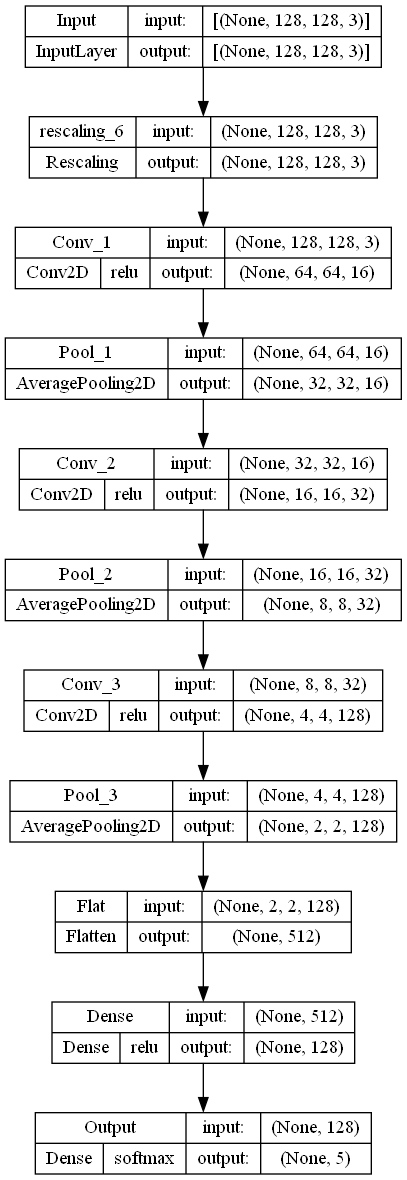
\includegraphics[scale=.45]{./p1-11}
    \caption{گراف مصور مدل}\label{fig.111}
\end{figure}

\begin{figure}[!h]
    \centering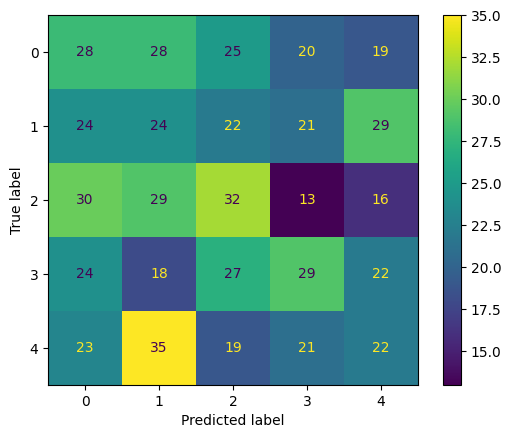
\includegraphics[scale=.70]{./p1-12}
    \caption{ماتریس درهم‌ریختگی}\label{fig.112}
\end{figure}

\begin{figure}[!h]
    \centering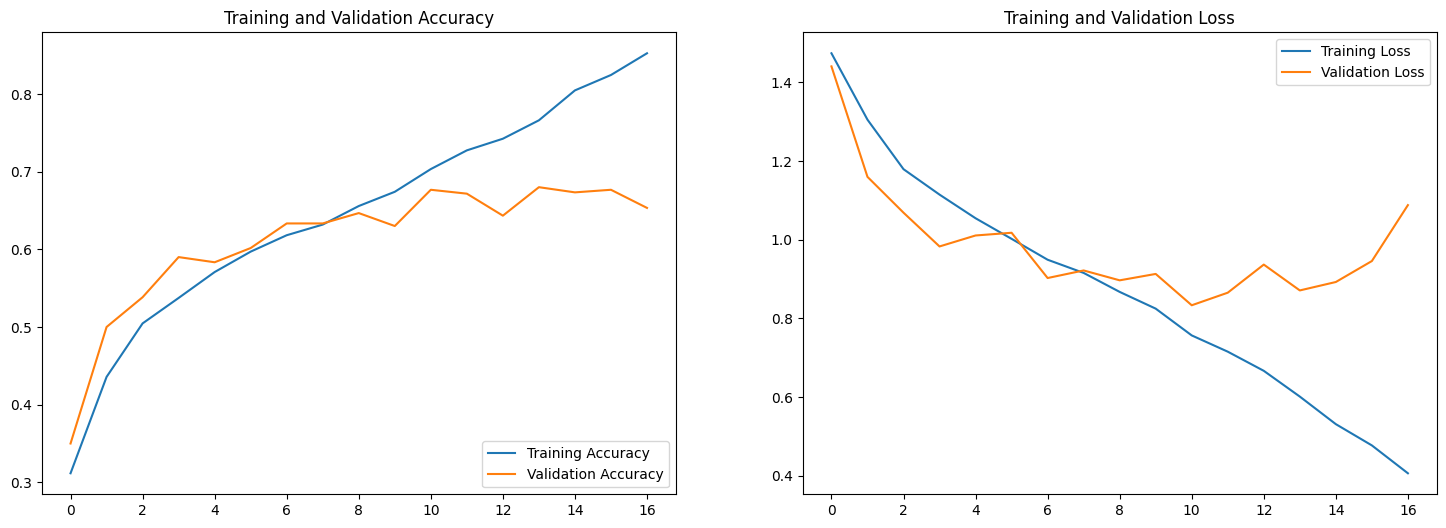
\includegraphics[scale=.45]{./p1-13}
    \caption{نمودارهای خطا و صحت}\label{fig.113}
\end{figure}

\cleardoublepage

همانطور که قابل مشاهده است، مقدار ای‌پاک 13 مقدار قابل قبولی خواهد بود. بعد از آن مدل دچار بیش‌برازش می‌شود.

برای مدل دوم گراف مصور مدل، ماتریس درهم‌ریختگی، نمودارهای خطا و صحت به ترتیب آورده شده‌اند.

\begin{figure}[!h]
    \centering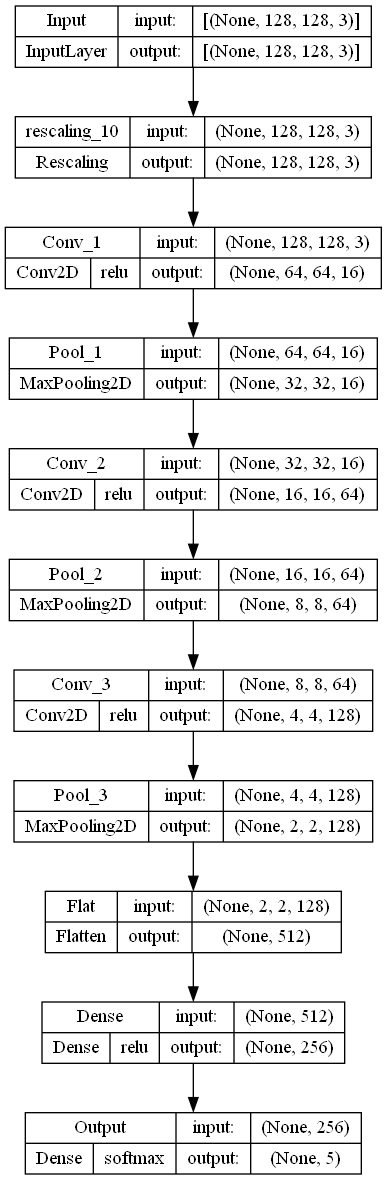
\includegraphics[scale=.45]{./p1-21}
    \caption{گراف مصور مدل}\label{fig.121}
\end{figure}

\begin{figure}[!h]
    \centering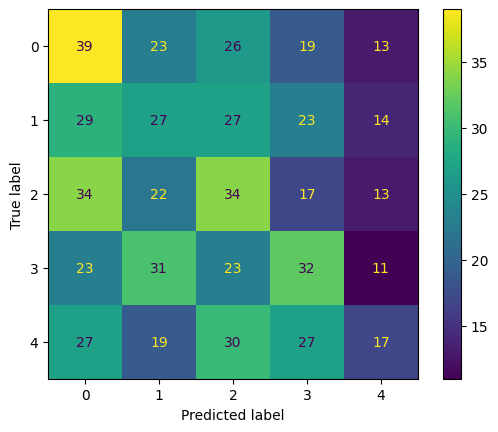
\includegraphics[scale=.70]{./p1-22}
    \caption{ماتریس درهم‌ریختگی}\label{fig.122}
\end{figure}

\begin{figure}[!h]
    \centering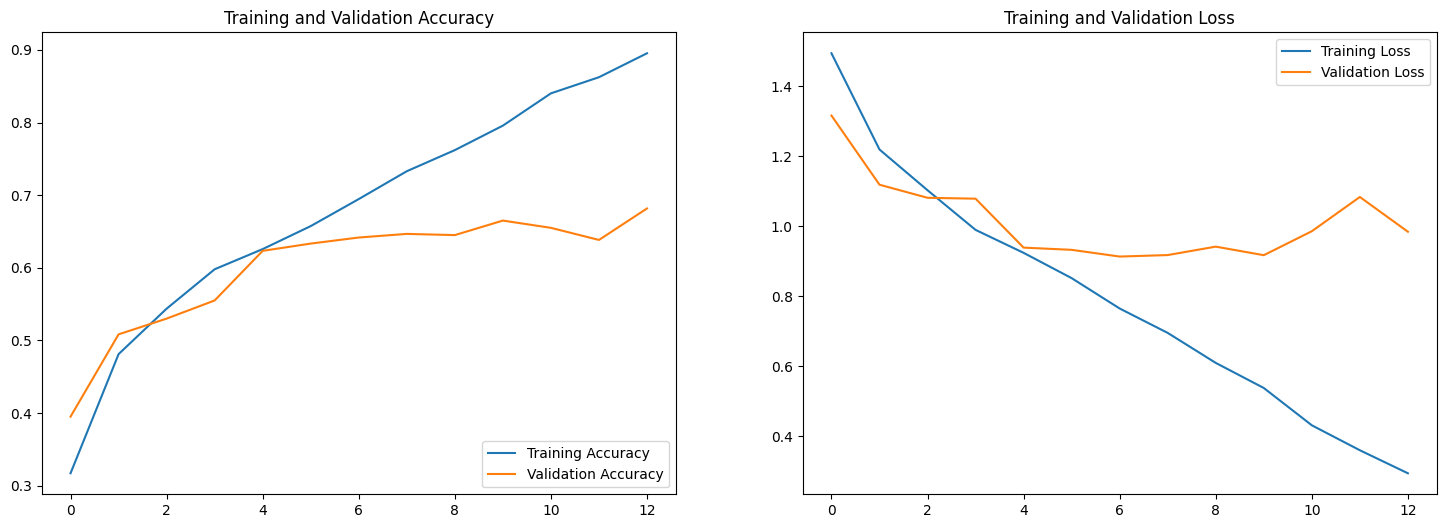
\includegraphics[scale=.45]{./p1-23}
    \caption{نمودارهای خطا و صحت}\label{fig.123}
\end{figure}


\cleardoublepage

همانطور که قابل مشاهده است، مقدار ای‌پاک 6 تا 9 مقدار قابل قبولی خواهد بود. بعد از آن مدل دچار بیش‌برازش می‌شود.

% -------------------------------------------------------------------
\section{پیاده‌سازی - سوال سوم}

برای این بخش ابتدا از یکی از مدل‌های آموزش داده شده استفاده می‌کنیم. و لایه اول کانولوشنی به عنوان خروجی در نظر گرفته می‌شود. همچنین سه عکس از مجموعه آموزشی درنظر گرفته می‌شود که در ادامه آورده شده است.

\begin{figure}[!h]
    \centering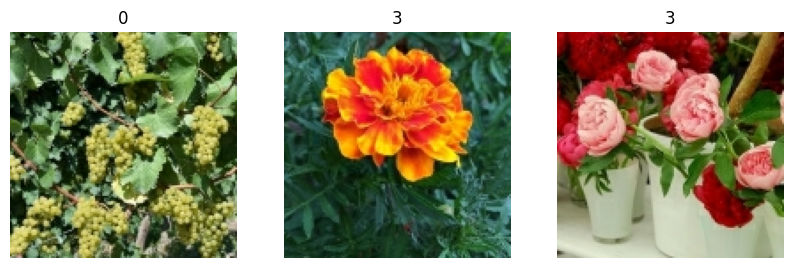
\includegraphics[scale=.45]{./p3-1}
    \caption{تصاویر انتخاب‌شده}\label{fig.31}
\end{figure}

\cleardoublepage

در ادامه نیز برای هر سه تصویر تعداد 16 فیلتر که برای لایه اول است آورده شده است. همانطور که مشاهده می‌شود، در اکثر فیلترها لبه‌ها و مرزها بوضوح قابل رویت هستند (حتی تصویر اول که انگوراست).


\begin{figure}[!h]
    \centering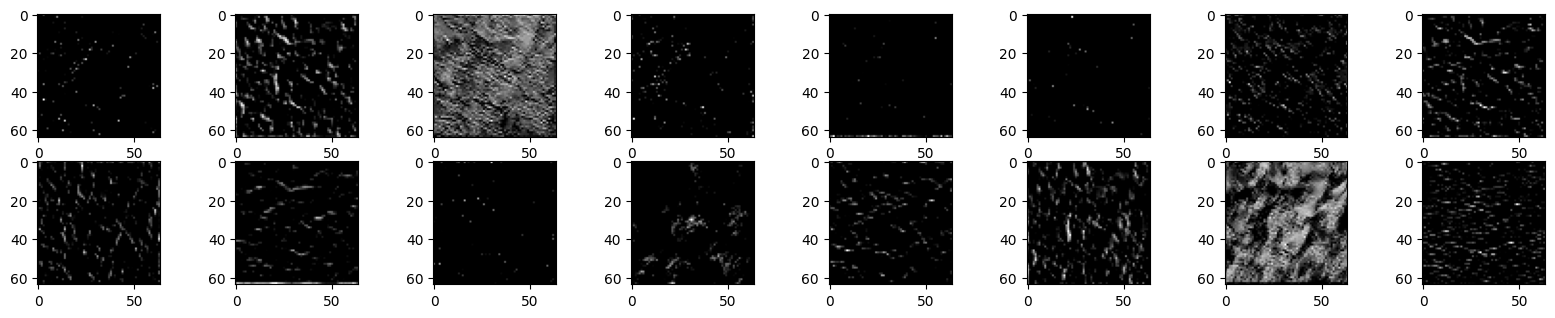
\includegraphics[scale=.40]{./p3-2}
    \caption{فیلترهای تصویر انگور}\label{fig.32}
\end{figure}

\begin{figure}[!h]
    \centering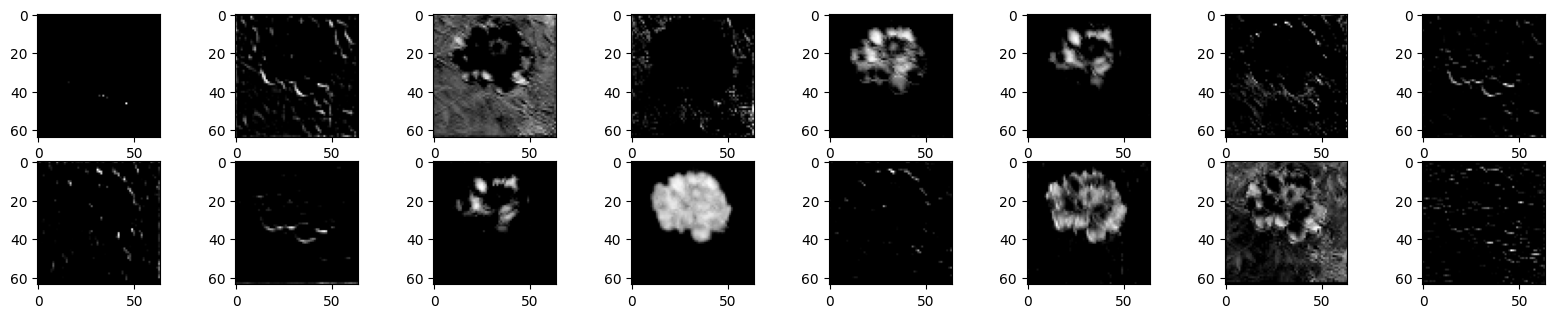
\includegraphics[scale=.40]{./p3-3}
    \caption{فیلترهای تصویر گل نارنجی}\label{fig.33}
\end{figure}

\begin{figure}[!h]
    \centering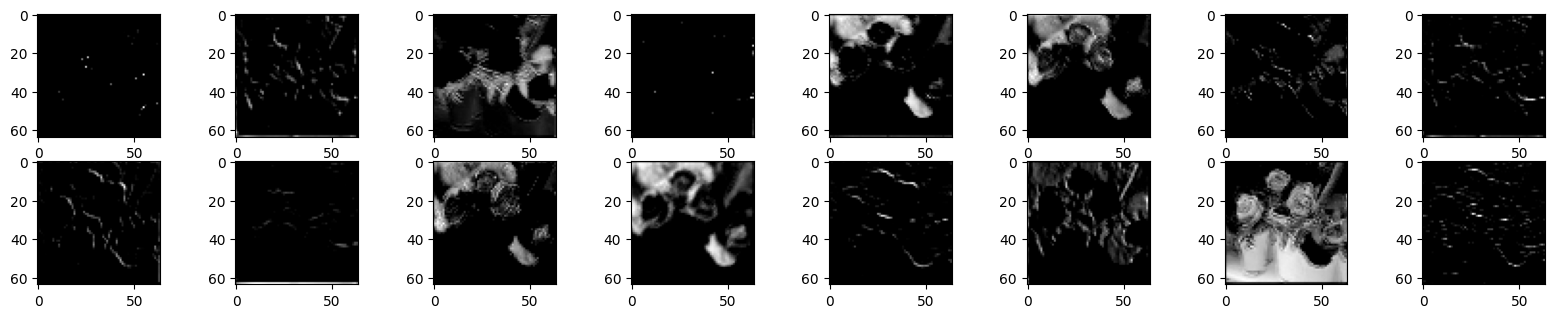
\includegraphics[scale=.40]{./p3-4}
    \caption{فیلترهای تصویر گل صورتی}\label{fig.34}
\end{figure}


\cleardoublepage

% -------------------------------------------------------------------
\section{پیاده‌سازی - سوال چهارم}
در این بخش نیاز است تا تعداد گام‌ها برابر با 1 باشد، تا معماری کار کند. به همین جهت معماری انتخاب شده برای این بخش شامل به ترتیب 16، 64 و 128 تعداد فیلتر با \lr{avg pooling} و همچنین 256 نورون لایه پنهان خواهد بود. ابتدا در ادامه معماری این قسمت مشاهده می‌شود. سپس ماتریس درهم‌ریختگی و درنهایت نمودارهای خطا و صحت نمایش داده می‌شود.

\begin{figure}[!h]
    \centering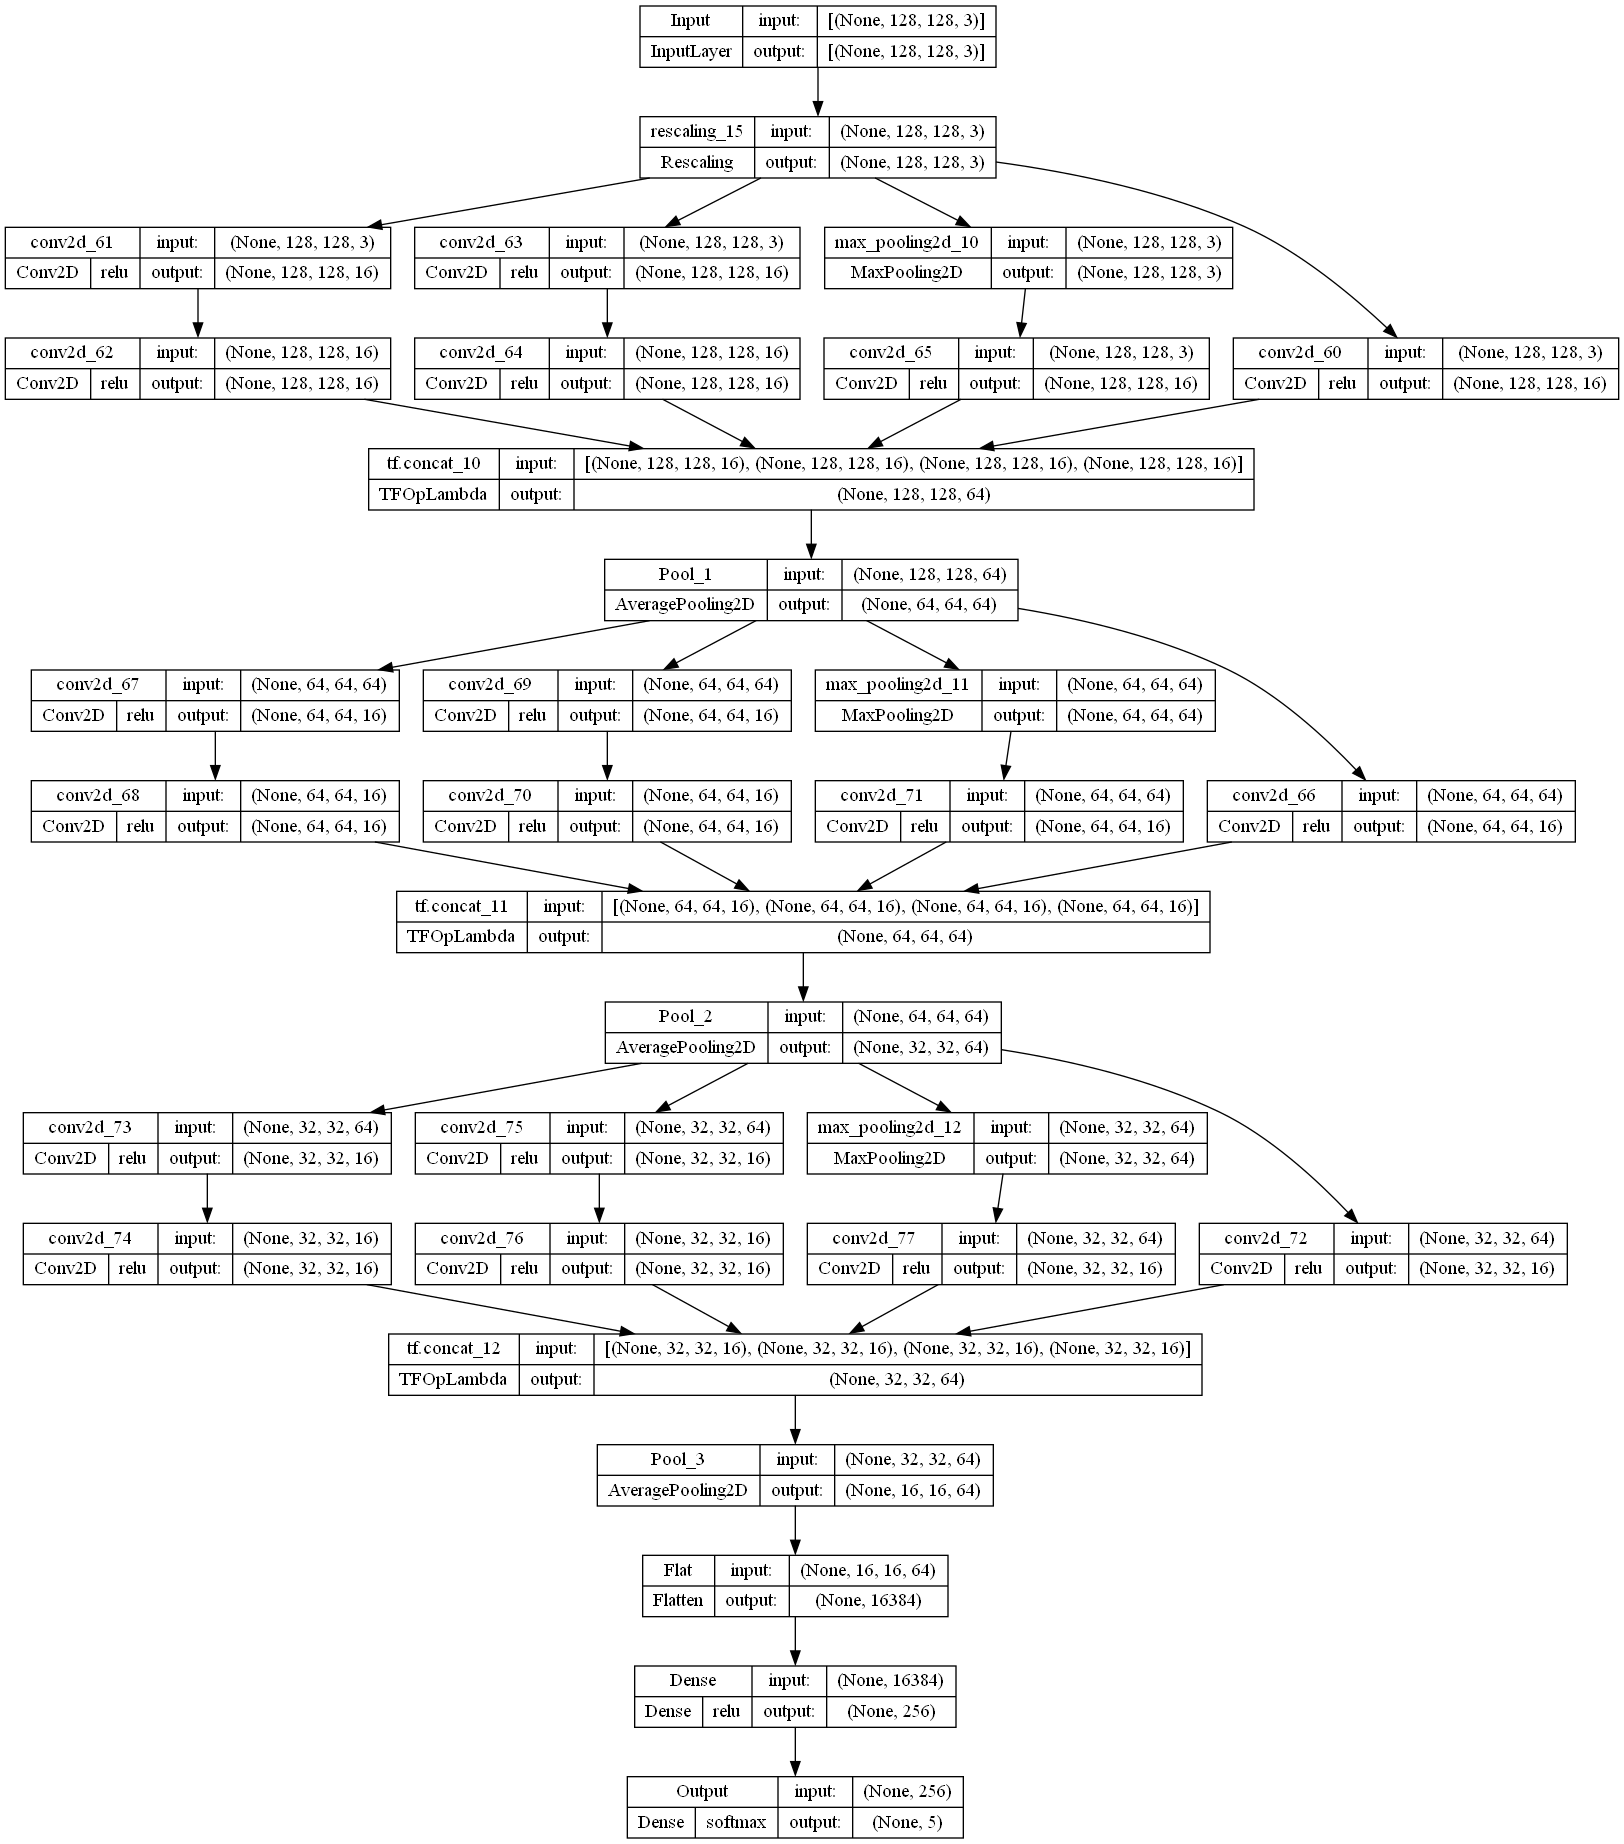
\includegraphics[scale=.25]{./p4-1}
    \caption{گراف مصور مدل}\label{fig.41}
\end{figure}

\begin{figure}[!h]
    \centering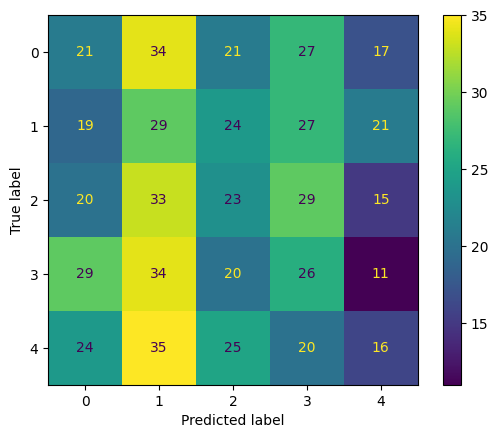
\includegraphics[scale=.70]{./p4-2}
    \caption{ماتریس درهم‌ریختگی}\label{fig.42}
\end{figure}

\begin{figure}[!h]
    \centering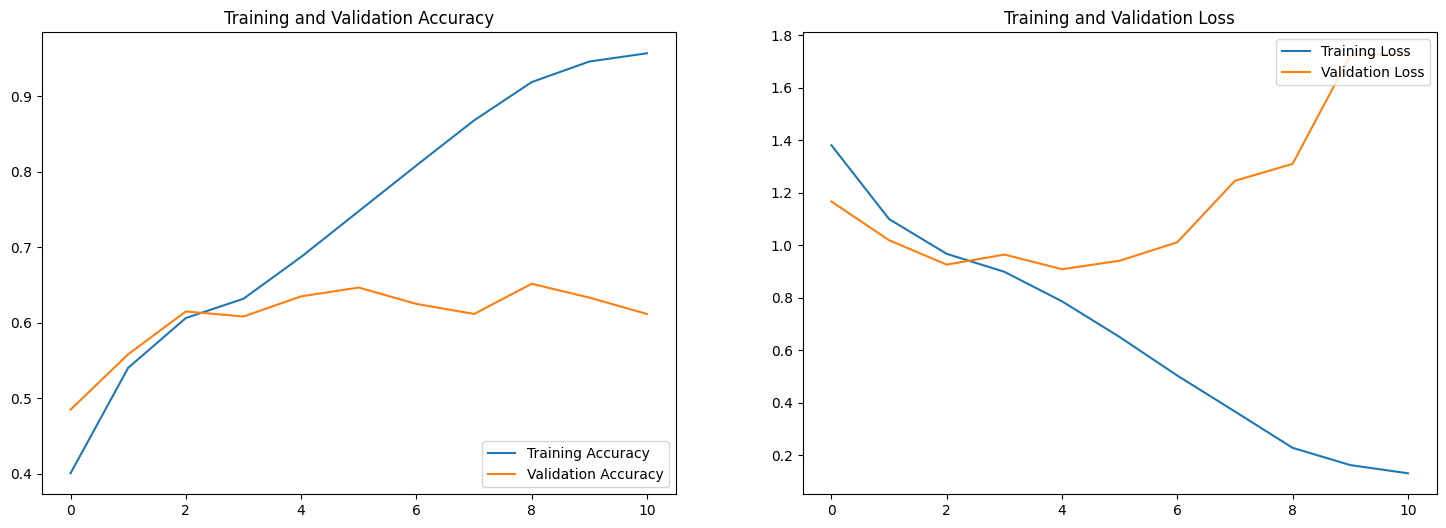
\includegraphics[scale=.45]{./p4-3}
    \caption{نمودارهای خطا و صحت}\label{fig.43}
\end{figure}

\cleardoublepage

اما نتایج گرفته شده جالب است. بر خلاف انتظار قبلی، در نتایج بهبودی خاصی در صحت مجموعه اعتبار سنجی وجود نداشت. بهترین صحت مجموعه اعتبار سنجی حدود 65 درصد بدست آمد (در مقایسه با 68 درصد در حالت اول (فایل ضمیمه)). از طرفی زمان آموزش بسیار طولانی‌تر شد (حدود 1 دقیقه و 45 ثانیه)، درحالیکه در حالت اولیه شبکه در حدود 17 ثانیه آموزش دید. این امر به دلیل افزایش چشمگیر پارامترهای آموزشی است. ولی نکته دیگر این شبکه زود به اتمام رسیدن آموزش آن توسط کالبک در مقایسه با حات اولیه بود. با شرایط یکسان در ای‌پاک 10 متوقف شد (درمقایسه با 12 و 16 ای‌پاک در حالت اولیه).


% -------------------------------------------------------------------
\section{پیاده‌سازی - سوال پنجم}

به دلیل آنکه مقادیر فیلتر‌ها با یک مجموعه آموزشی، آموزش دیده‌اند. به طور کلی وظایف فیلترها استخراج ویژگی‌ها (مانند لبه‌ها و مرزها) است. یک فیلتر مشخص برای هر عکس یک عملکرد مخصوصی دارد. همانطور که در سوال 3 مشاهده شد. لذا اساسا در ابتدا نیازی به آموزش نیست. از طرفی شباهت‌هایی نیز بین مجموعه‌های داده نیز وجود دارد (وجود گل‌ها در مجموعه داده اول). اما برای عملکرد بهتر در گام‌های بعدی آموزش قسمت استخراج ویژگی ادامه می‌یابد.

% -------------------------------------------------------------------
\section{پیاده‌سازی - سوال ششم}

هرچه پیچیدگی دسته‌بند بیشتر باشد نیاز است تا در گام اول یادگیری، ای‌پاک‌های بیشتری در نظر گرفته شود. زیرا با افزایش پیچیدگی پارامترها نیز افزایش یافته و زمان بیشتری نیاز است تا آموزش ببینند. اما طراحی معماری دسته‌بند در این مثال خاص با روش زیر طراحی شد.

با همان روش ذکر شده از تعریف پروژه، ابتدا قسمت استخراج ویژگی را برداشته (غیر قابل آموزش) و سپس مقادیر مختلفی از تعداد نورون دسته‌بند با مقدار ای‌پاک 15 آموزش می‌دهیم. سپس بهترین مقدار صحت مجموعه اعتبارسنجی را در نظر گرفته و مقدار متناظر نورون آن را انتخاب می‌کنیم. درنهایت همه پارامترهای استخراج ویژگی را قابل آموزش‌دهی کرده و آموزش را از سر می‌گیریم.


جدول زیر مقدار صحت مجموعه آموزش و اعتبارسنجی به ازای تعداد نورون را نشان می‌دهد.

\begin{table}[h!]
    \centering
    \begin{tabular}{|c|c|c|c|}
    \hline
    نورون & آموزش صحت & اعتبارسنجی صحت & تست صحت\\ \hline
    16 & $43.28$ & $46.24$ & $43.28$\\ \hline
    32 & $44.99$ & $43.23$ & $45.97$\\ \hline
    64 & $49.71$ & $48.7$ & $47.58$\\ \hline
    128 & $50.33$ & $47.61$ & $48.92$\\ \hline
    256 & $52.12$ & $49.25$ & $50.27$\\ \hline
    \end{tabular}
    \end{table}

\cleardoublepage

همانطور که مشاهده می‌شود بهترین تعداد نورون 256 تا است. در ادامه آموزش را به ازای 256 نورون تکمیل کرده و خروجی مشاهده می‌شود.

برای مدل نهایی گراف مصور مدل، ماتریس درهم‌ریختگی، نمودارهای خطا و صحت به ترتیب آورده شده‌اند.

\begin{figure}[!h]
    \centering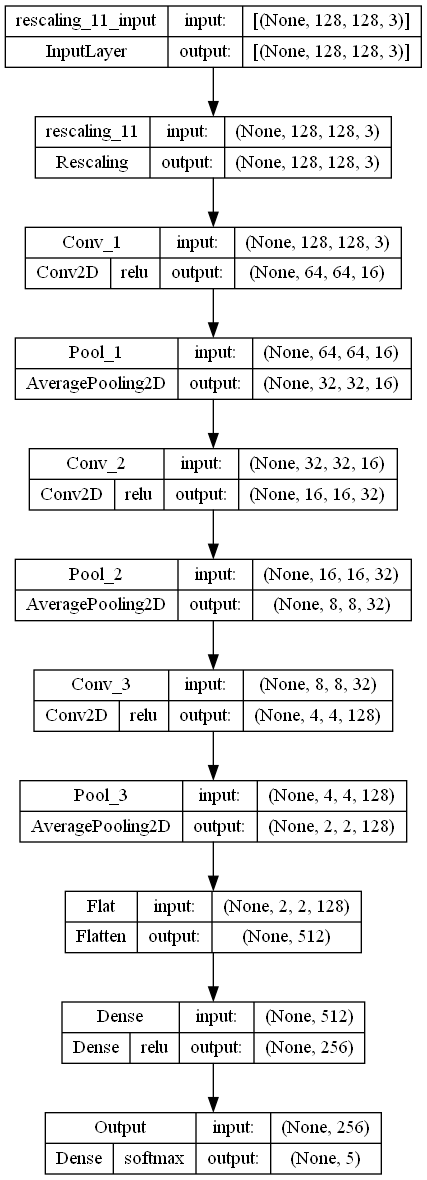
\includegraphics[scale=.45]{./p6-1}
    \caption{گراف مصور مدل}\label{fig.61}
\end{figure}

\begin{figure}[!h]
    \centering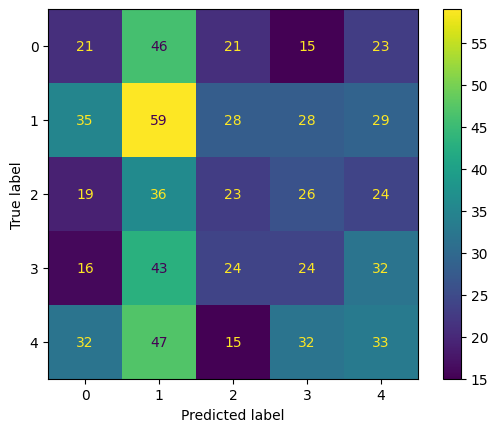
\includegraphics[scale=.70]{./p6-2}
    \caption{ماتریس درهم‌ریختگی}\label{fig.62}
\end{figure}

\begin{figure}[!h]
    \centering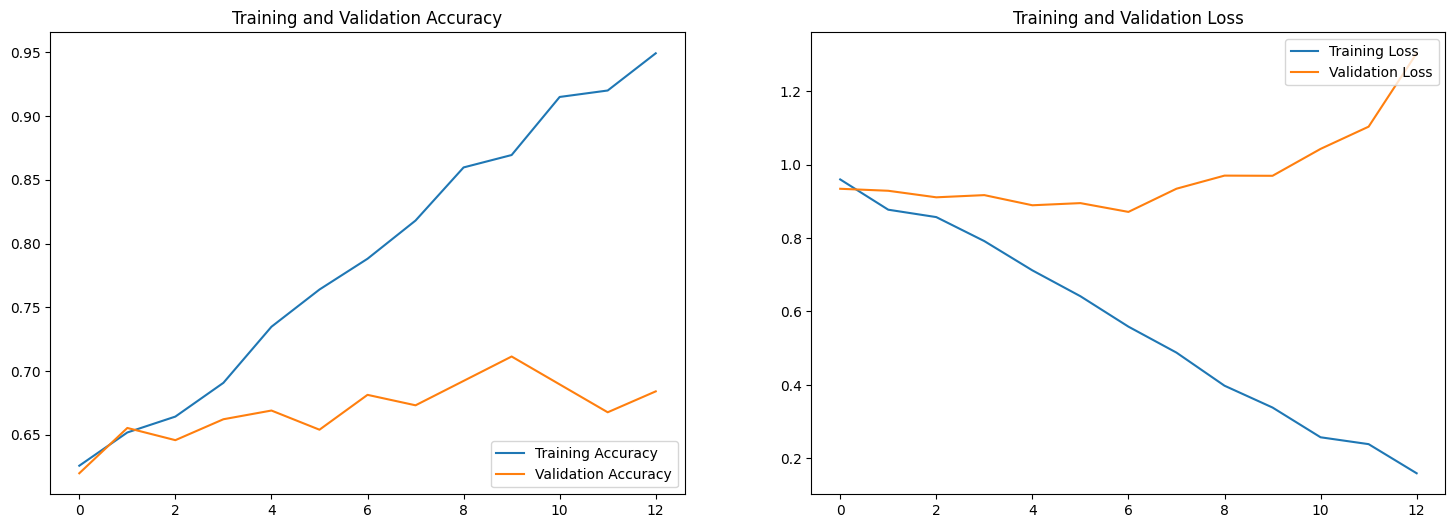
\includegraphics[scale=.45]{./p6-3}
    \caption{نمودارهای خطا و صحت}\label{fig.63}
\end{figure}

\cleardoublepage

همانطور که مشاهده می‌شود، نتایج نیز در بهترین حالت در ای‌پاک 9 با 70 درصد صحت اعتبارسنجی رخ داد، که بعد از آن مدل رفته رفته دچار بیش‌برازش شد.


% -------------------------------------------------------------------

% -------------------------------------------------------------------

\end{document}